% paper.tex — preprint source, generated 2026-10-14 from 04_manuscript.md (Paper 2,
% "Fitting the Practice, Not the Works: A Human-Referential Theory of AGI").
% Build: any LaTeX toolchain that runs BibTeX (pdflatex -> bibtex -> pdflatex x2),
%        or `tectonic paper.tex` in this directory (requires references.bib + figures/).
% For arXiv upload: include the generated paper.bbl (arXiv does not run BibTeX).
%
% NOTE(submission): self-description is "a theory paper = conceptual synthesis +
% a structured literature audit" (original research: new coding instrument, an
% 80-work coded corpus released as data, exact-binomial and Fisher results, and a
% registered absence-search procedure) — NOT a "position paper" or "review"; see
% 05_submission_package.md §1.3 (arXiv cs moderation practice of 2025-10-31).
%
% CJK note: two CJK strings appear (Sec.~6 gloss; three Chinese policy-document
% titles in the bibliography). xeCJK + Songti.ttc is configured below for macOS;
% on Linux replace with e.g. Path to Noto Sans CJK SC. If xeCJK is unavailable,
% the two strings can be romanized without loss of cited content.

\documentclass[10pt]{article}

\usepackage[margin=1in]{geometry}
\usepackage[T1]{fontenc}
\usepackage[utf8]{inputenc}
\usepackage{amsmath}
\usepackage{newtxtext,newtxmath}
\usepackage{microtype}
\setlength{\emergencystretch}{2em}
\usepackage{graphicx}
\graphicspath{{figures/}}
\usepackage{booktabs}
\usepackage{array}
\usepackage[numbers,sort&compress]{natbib}
\usepackage{xcolor}
\usepackage{xeCJK}
\setCJKmainfont[Path=/System/Library/Fonts/Supplemental/,Extension=.ttc]{Songti}
\usepackage[colorlinks=true,linkcolor=blue!60!black,citecolor=blue!60!black,urlcolor=blue!60!black]{hyperref}
\urlstyle{same}

\newcommand{\dminus}{-}

\title{\textbf{Fitting the Practice, Not the Works:\\
A Human-Referential Theory of AGI}}

\author{Yugui Yu\\
YYG Strategy Lab\\
\texttt{they4897@gmail.com}
% TODO(user): add ORCID before submission
}
\date{}

\begin{document}
\maketitle

\begin{abstract}
\noindent This paper proposes a human-referential fitting theory of artificial general intelligence (AGI) --- in Chinese, AGI 人本拟合论 --- and makes it testable through a structured coding audit of 80 training-objective works. The theory advances three connected claims. Conceptually, AGI is a philosophical concept: as long as ``generality'' is referenced to the open set of human practice, it cannot be reduced to a technical specification. In implementation, the means of AGI is the fitting of human practice --- not the fitting of humanity's accumulated works. Normatively, AGI should be positioned as an augmentative tool, not a new subject. The theory's core is a temporal clause: \emph{The object of fitting is not humanity's works but its practice --- the full spectrum and the full course of human experience. The stock has a wall; the flow does not.} The audit codes a purposefully sampled corpus of $N = 80$ works on two stance axes (descriptive and normative) and eight fitting-object dimensions; its principal result quantifies the theory's central gap: the experience-type axis (success/failure, expert/novice, typical/marginal) is explicitly treated in 0/80 works (exact binomial 95\% CI $[0.0\%, 4.5\%]$), while practice-as-flow is explicit in only 2/80 works, both from 2026; works-as-stock shows continuous explicit treatment from 2022 onward, and output-distribution coverage first appears in 2024. We derive the theory's methodological implications for distribution, production, and governance, and state falsification conditions.
\end{abstract}

\medskip
\noindent\textbf{Keywords:} artificial general intelligence; practice-fitting; human-referential fitting; data walls; augmentation; evidence mapping

\section{Introduction}\label{sec:intro}

Every frontier model is, among other things, a distillation of what humans have produced --- web text, code, mathematics, ratings. The phrase ``trained on human data'' is so familiar that its ambiguity goes unnoticed. It admits two readings that diverge into different research programs. On the static reading, the fitting object is humanity's \emph{works}: a finite, already-produced archive that can be crawled, cleaned, deduplicated, and exhausted. On the dynamic reading, the fitting object is humanity's \emph{practice}: the ongoing regeneration of experience --- tool use, interaction, feedback, failure, repair --- which continues as long as life continues. We call the first \emph{corpus-fitting} and the second \emph{practice-fitting}; the theory itself we name the \emph{human-referential fitting theory} of AGI (Chinese: AGI 人本拟合论) --- \emph{human-referential} marks the reference frame, \emph{fitting} the means. The static reading currently dominates: scaling analyses reason about the finite stock of public human-generated text (estimated at roughly 300 trillion tokens \cite{villalobos2022data}); flagship technical reports document static mixture ratios over archived corpora \cite{grattafiori2024llama3}. The dynamic reading is the reading this paper defends.

The distinction is fixed by a single sentence, which we call the temporal clause and which guards the theory against its most likely misreading:

\begin{quote}
\textbf{The object of fitting is not humanity's works but its practice --- the full spectrum and the full course of human experience. The stock has a wall; the flow does not.}
\end{quote}

Two axes compose the fitting target. The \emph{full spectrum} is the cross-sectional axis: who is represented, and which kinds of experience --- success and failure, expert and novice, typical and marginal. The \emph{full course} is the longitudinal axis: the time stream of practice, which no snapshot archives. The stock/flow asymmetry has a precise meaning in this theory: the data wall \cite{villalobos2022data} is a property of the stock, not an anthropological limit; model collapse under recursive training on generated data \cite{shumailov2024collapse} is a pathology of treating the stock as if it were self-renewing. Flow-side data --- production telemetry, interaction logs, failure submissions --- regenerates with deployment. The philosophical skeleton of the distinction is Arendt's tripartition of labor, work, and action \cite{arendt1958human}: the static misreading fits only the products of \emph{work}, while this theory takes the ongoing processes of labor and action as the fitting object.

This paper builds on a prior empirical audit \cite{yu2026failure}, which examined how the industry handles failure data across the model-training lifecycle and documented its systematic discard. That audit measured what the stock discards; the present paper states the theory --- the training object is practice, not works: the turn from stock to flow. How to collect, clean, and absorb the flow is future work.

\paragraph{Gap.}
Four literatures are individually mature but unconnected. Cultural-technology analyses tell us what large models \emph{are} --- technologies that inherit the structure of human symbolic production \cite{farrell2025cultural}. Critical phenomenology tells us what models \emph{reflect} --- a distorting mirror that shapes human self-understanding \cite{vallor2024mirror}. Augmentation economics tells us what AI \emph{should be} --- a complement to human agency rather than a substitute for it \cite{brynjolfsson2022turing}. Pluralistic alignment tells us \emph{whose values} should be fitted \cite{gabriel2020values}. What is missing is the connective proposition that unifies them --- fitting human practice as the means, augmenting humans as the end --- together with the temporal concept tool (stock vs.\ flow) that the data-methodology debate lacks. A metrological literature, meanwhile, warns that our benchmarks are sampling projections of human practice and often poor ones \cite{salaudeen2025measurement}, which makes the reference-frame question unavoidable rather than rhetorical.

\paragraph{A note on terminology.}
\emph{Fitting} is used here in the statistical sense (approximating a distribution or functional structure) extended to a total object: the expressible projections of human forms of life. It is broader than \emph{imitation} (behavioral matching) and narrower than \emph{alignment} (a normative relation). Unlike \emph{mimicry}, fitting does not presume the goal of passing as human. The theory will argue, in fact, that fitting is a \emph{means} that fails as an \emph{end}.

\paragraph{Contributions.}
This paper makes four contributions:
\begin{enumerate}
\item \textbf{A temporal distinction} between fitting humanity's works and fitting humanity's practice, stated as the temporal clause with named terminology (corpus-fitting vs.\ practice-fitting; full spectrum $\times$ full course; fitting lag --- the gap between daily practice regeneration and periodic model snapshots).
\item \textbf{A coordinate system} for the fitting target --- the full-spectrum $\times$ full-course plane --- identifying experience type as the coverage axis missing from current practice, beyond the two existing axes of population (who) and output distribution.
\item \textbf{A structured evidence map} --- a methodological component in the spirit of the companion audit's codebook \cite{yu2026failure} --- that turns the theory's central gap into a quantifiable, falsifiable result: the experience-type axis is explicitly treated in 0 of 80 works.
\item \textbf{Four termination boundaries} for flow-side fitting (end of the practicing subject; fitter overreach; institutional boundary; self-referential contamination), which convert the temporal clause from a slogan into a bounded claim.
\end{enumerate}

\paragraph{Roadmap.}
Section~\ref{sec:concept} argues that AGI is a philosophical concept. Section~\ref{sec:implementation} develops practice-fitting as the implementation thesis, treating three lines of opposition head-on, and closes with a formal sketch (Section~\ref{sec:formalsketch}) that renders the stock/flow distinction as a pair of optimization problems and the boundaries as stopping conditions. Section~\ref{sec:position} states the augmentative-tool stance as a normative stance with an academic lineage. Section~\ref{sec:evidencemap} presents the evidence map: method, tables, figures, and the quantified gap. Section~\ref{sec:concurrent} consolidates the demarcation against adjacent frameworks, architecture-side programs, and concurrent works. Section~\ref{sec:tensions} addresses the tensions and fixes the four boundaries. Section~\ref{sec:implications} derives three methodological implications for future work. Section~\ref{sec:conclusion} concludes.

\section{Concept: AGI as a Philosophical Concept}\label{sec:concept}

The theory's first claim is conceptual: AGI is not an engineering specification awaiting completion but a philosophical concept whose reference frame is human practice. Three streams of literature converge on this.

\paragraph{The definition genealogy is itself philosophical.}
Legg and Hutter define universal intelligence as goal achievement across a wide range of environments --- generality indexed by environmental scope \cite{legg2007universal}. The Levels-of-AGI framework operationalizes generality $\times$ autonomy into a taxonomy of levels \cite{morris2023levels}. The METR task-length benchmark measures the time horizon of tasks an AI can complete, with doubling-time estimates of roughly seven months across the full series \cite{kwa2025measuring}, revised toward about four months over 2023--2026 in its 2026 update \cite{metr2026th11} --- an update whose maintainers themselves flag ceiling saturation of the task suite, and which a published critique argues cannot support strong conclusions, citing contamination risks in the task suite and the narrowness of the human baselines \cite{witkin2026metr}. We therefore use time horizon as one fallible proxy among the operationalizations below, not as a load-bearing premise. These operationalizations are useful, but each inherits its notion of ``general'' from an implicit sampling of environments --- and environments, for AI systems, are human-built situations of use. The operationalizations are proxies for a concept they do not define.

\paragraph{The metrological critique is decisive on this point.}
A validity-centered framework for AI evaluation imports construct validity from psychometrics and finds most benchmarks unable to support the claims built on them \cite{salaudeen2025measurement}. Parallel work in the psychometrics tradition shows that apparent cognitive-like capabilities in language models are sensitive to item interrelatedness and measurement design \cite{ilic2024evidence}, and that psychometrically derived short benchmarks change the rank ordering of the same models \cite{gignac2025psychometrically}. The shared implication is that benchmark tasks are \emph{sampling projections of human practice}: a benchmark is general only relative to the slice of practice it samples. A concept whose operationalization is a sample of practice cannot float free of the practice it samples.

\paragraph{The moving-target critique converges from the other side.}
Tesler's theorem --- intelligence is whatever machines have not done yet --- describes the definitional recession that has accompanied AI since its founding \cite{tesler1997effect}; a recent essay presses the analogy between AGI and a perpetual-motion machine, a category error rather than a hard goal \cite{imeri2025benefits}; and a rigor-oriented analysis argues that AI progress talk systematically lacks the inferential discipline of mature sciences \cite{nguyen2026rigor}. If AGI were a fixed technical target, these pathologies would be curable by better measurement. On the view defended here, they are symptoms of the concept's true structure: as long as ``general'' references the open set of human practice, AGI cannot be specification-grade, because the reference set is open and moving --- not because intelligence is mysterious.

\paragraph{Philosophical anthropology supplies the positive anchor.}
Plessner's law of natural artificiality holds that the human being is constitutively artificial --- an organism that completes itself through artifacts, excentrically positioned toward its own nature \cite{plessner1928levels}. On this anthropology, tool-use is not a rupture of human nature but its normal mode; readings of Plessner in the age of media technologies extend exactly this point to digital artifacts \cite{demul2014philosophical}, and the ``Homo Translator'' analysis of human-in-the-loop bio-inspired technologies makes the human--artifact circuit explicit \cite{tamborini2025homo}. The tool stance defended in Section~\ref{sec:position} therefore does not need to apologize for being ``merely instrumental'': instrumentality is an anthropological constant, not a metaphysical demotion. What Plessner adds over both boosterism and anxiety is a criterion: the question is not whether humans use artifacts to complete themselves (they always have), but whether this artifact is fitted to the full range of what humans do --- including how humans err.

Figure~\ref{fig:framework} summarizes the theory in this coordinate system: the fitting object runs from works (static stock, bounded by the wall) to practice (regenerating flow); the vertical axis is the full course of practice; the flow region carries the two existing coverage axes and marks the missing third; four boundaries terminate the fit.

\begin{figure}[t]
\centering
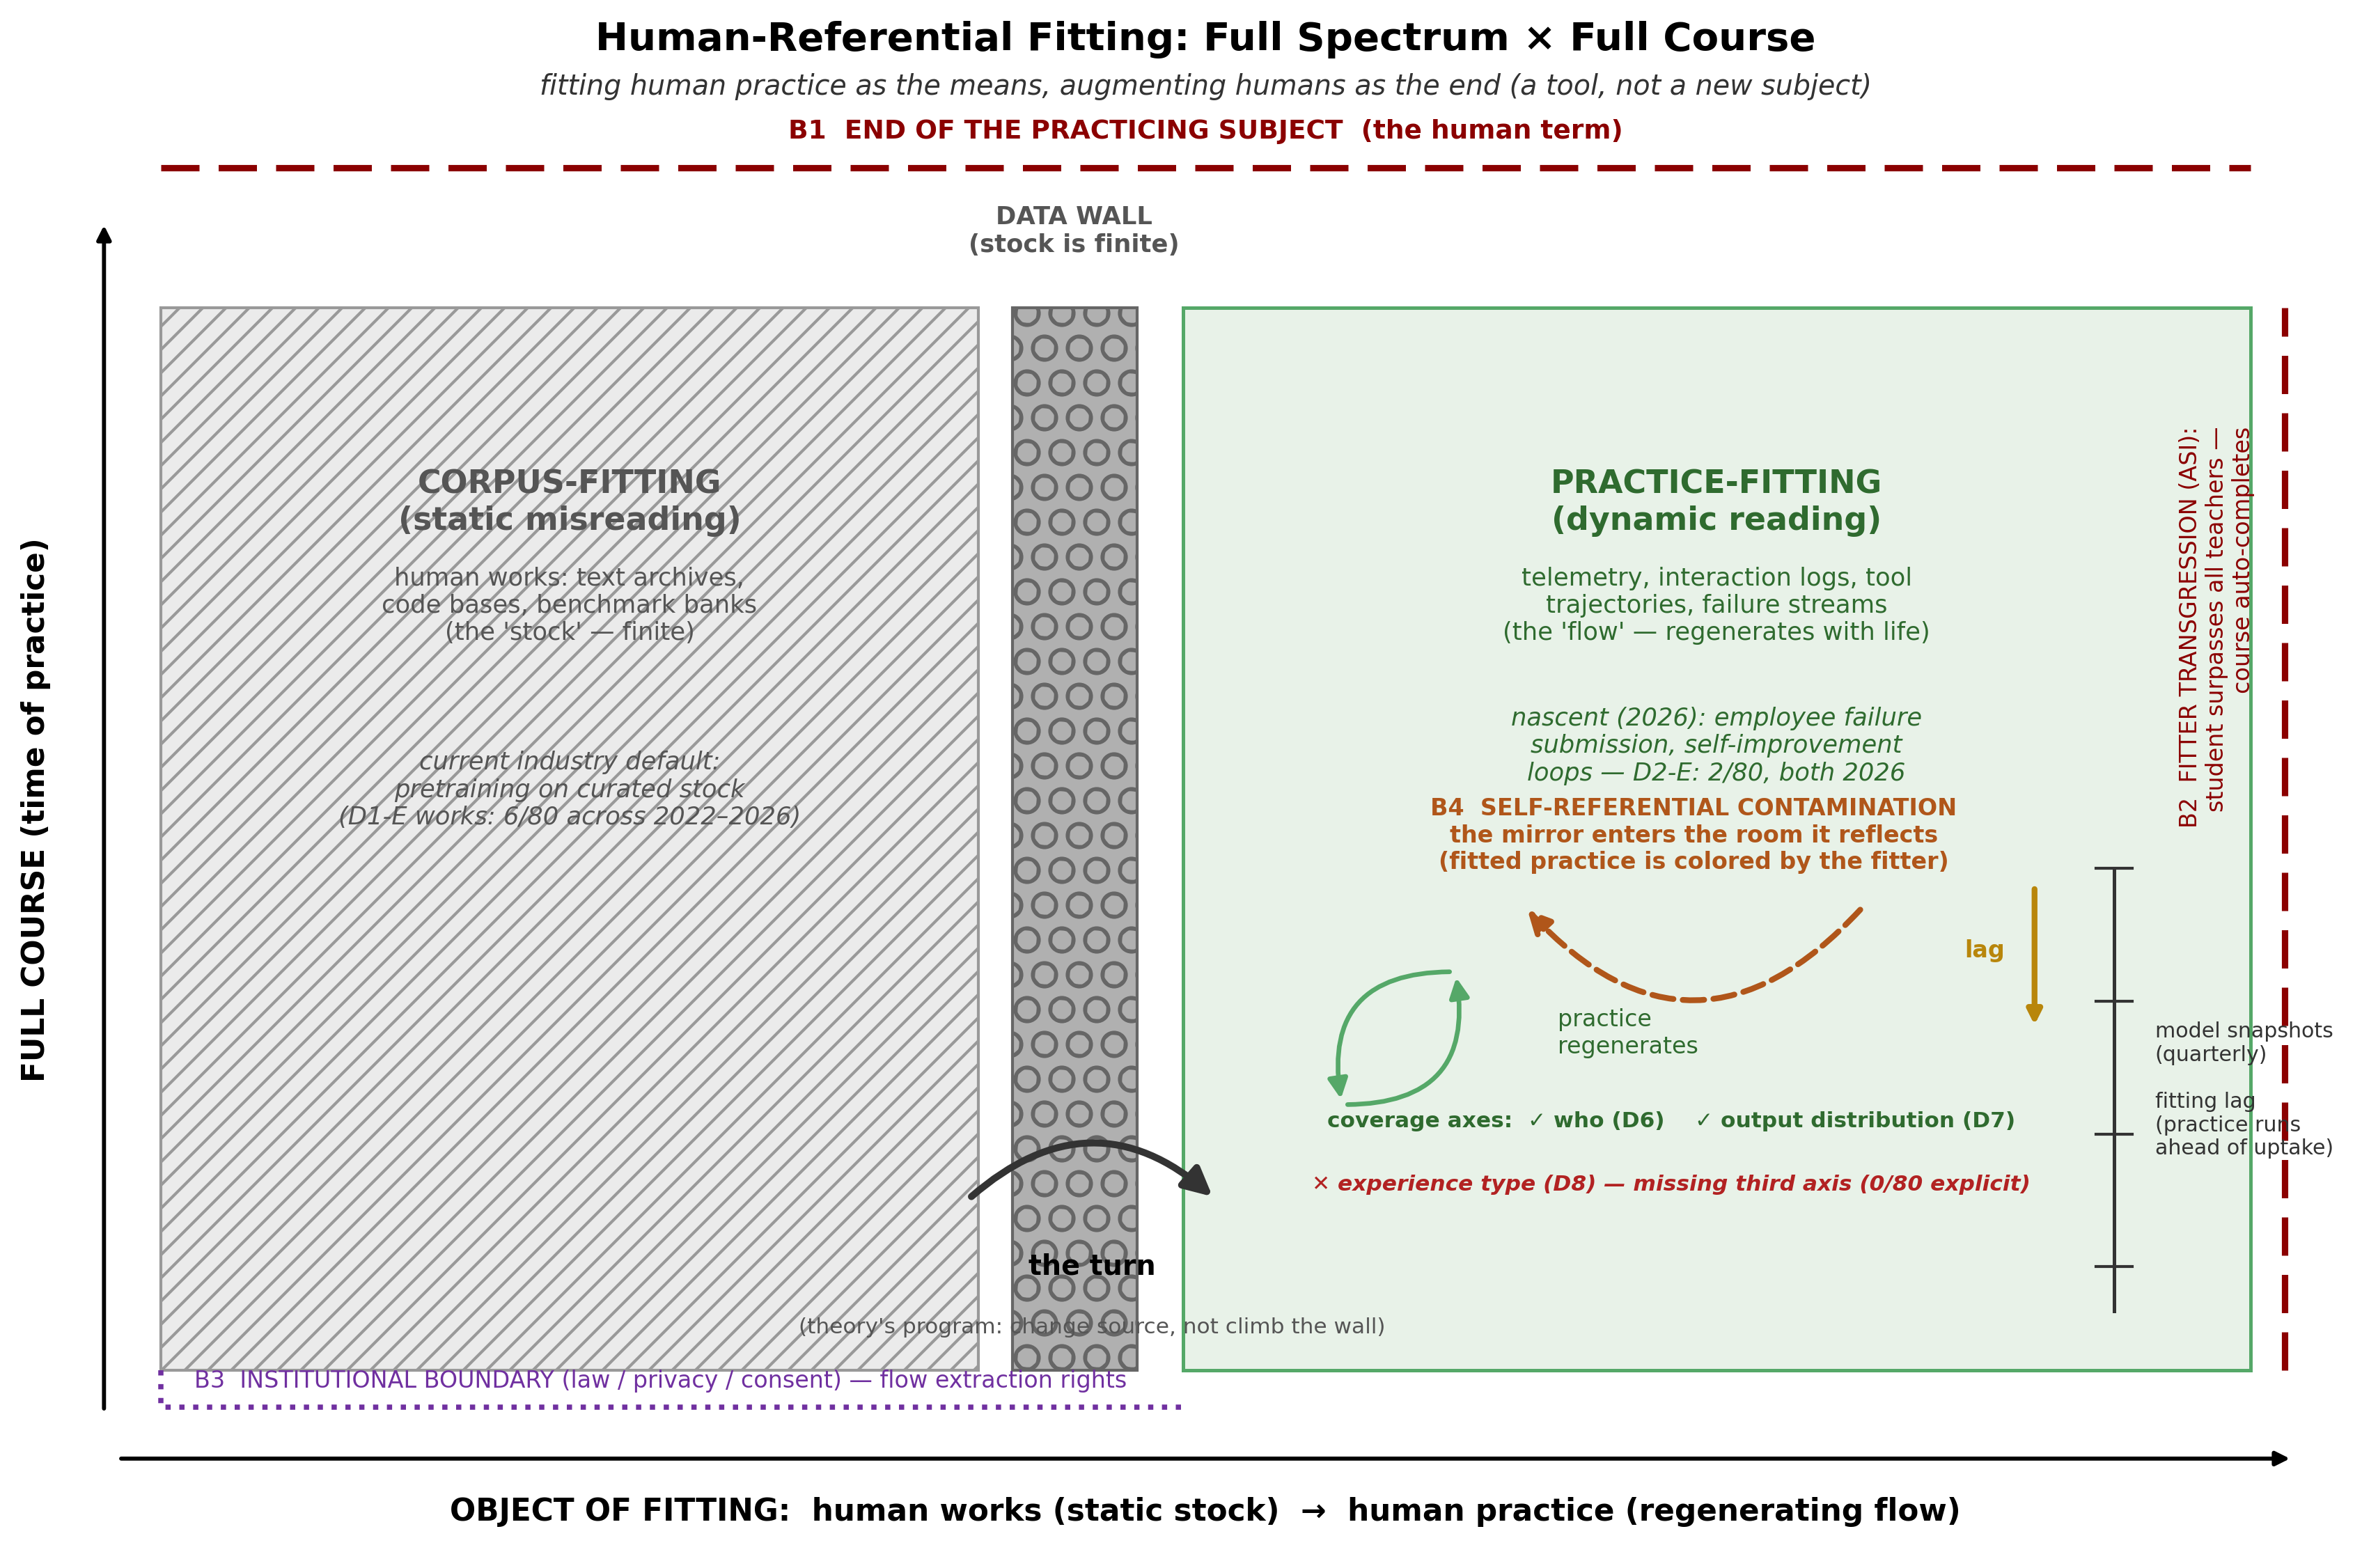
\includegraphics[width=\textwidth]{fig1_theory_framework.png}
\caption{The theory at a glance: the full-spectrum $\times$ full-course coordinate system. Horizontal axis: the fitting object, from humanity's works (static stock; brick pattern = the data wall) to humanity's practice (regenerating flow; circular arrows). Vertical axis: the temporal course of practice. Within the flow region, the two existing coverage axes are annotated (who/population, D6; output distribution, D7) together with the missing third axis (experience type, D8; 0/80 works in our corpus). Right margin: the fitting-lag timeline --- practice regenerates continuously while model snapshots update periodically. The four termination boundaries are marked: B1, end of the practicing subject (top, dashed); B2, fitter overreach (right; the fitting relation exhausts itself --- no practice remains that is not already behind it); B3, institutional boundary (bottom, dotted; law, privacy, consent); B4, self-referential contamination (return arc; ``the mirror enters the room it reflects''). The central ``turn'' arrow crosses \emph{beyond} the wall --- changing the source rather than climbing it. Subtitle: fitting as the means, augmenting as the end (a tool, not a new subject).}
\label{fig:framework}
\end{figure}

The convergence of the three streams yields the first claim. The definitional genealogy cannot close the concept; the measurement critique shows the operationalizations are practice-samples; the moving-target critique explains why; and philosophical anthropology blocks the inference that ``unspecifiable'' means ``hostile to technology.'' AGI as a human-referential concept is a lens, not a countdown.

\paragraph{The intelligence--practice relation, stated as such.}
These claims jointly fix the theory's stance on the relation between intelligence and practice, and we state it as a proposition. Definitionally, generality is not a self-contained intrinsic property but a relational one: a system counts as ``general'' only relative to the open set of human practice it is referenced against --- which is why every operationalization above is a sampling projection of practice rather than an intrinsic measure. Developmentally, such intelligence is acquired by fitting practice and kept current by practice's regeneration: practice regenerates daily while model snapshots update on cycle, and the fitting lag (Section~\ref{sec:formalsketch}) is the distance-metric of this relation --- how far the fitted intelligence has fallen behind the practice that defines it. Ontologically, practice precedes works: works are frozen, biased projections of practice, so the choice of fitting object is not a data-engineering preference but a content-determination of the intelligence concept itself. The implementation claim of Section~\ref{sec:implementation} operationalizes this triple relation, and the theory's name marks it: the reference of fitting is humans-as-practicing, not minds-replicated. The concept also packs two human demands with distinct references --- \emph{generality}, which references the open set of practice, and \emph{height}, which references the performance of human teachers; both are demand-side specifications, which is why AGI is a lens on what humans need rather than a specimen description of what machines are.

\section{Implementation: Practice-Fitting as the Means}\label{sec:implementation}

The second claim is implementational: the path to AGI runs through the fitting of human practice --- its knowledge, norms, functional emotion-motivation structures, and failure modes --- and this fitting is \emph{means}, not end.

\paragraph{The cultural-technology thesis sets the frame.}
Farrell, Gopnik, Shalizi, and Evans argue in \emph{Science} that large AI models are cultural and social technologies: like writing and markets, they inherit, transmit, and recombine the structure of human symbolic production, with the pathologies such transmission entails \cite{farrell2025cultural}. The cognitive line corroborates: children's cultural learning through imitation exhibits transmission-versus-truth trade-offs that current models handle differently \cite{yiu2024transmission}; large models spontaneously develop human-like analogical reasoning from text alone \cite{webb2023emergent}. If models are cultural technologies, their competence is inherited from human practice --- which makes the \emph{quality of the inheritance} (what is transmitted, from whom, including error) the central engineering variable, not an afterthought.

\paragraph{The empirical chain is no longer speculative.}
GPT-4o reproduces human-like patterns of cognitive dissonance and self-justification moderated by free choice \cite{lehr2025kernels}; generative models exhibit human-like social identity biases \cite{hu2025generative}; and interpretability work has identified causally functional emotion concepts inside a production model, influencing its outputs and its conception of its own role \cite{anthropic2026emotions}. On the value side, cooperative inverse reinforcement learning formalizes the AI--human relation as assistance with an unknown human reward function \cite{hadfield2016cooperative}; preference learning trains reward models that are, structurally, fitters of human preference distributions \cite{christiano2017deep, ouyang2022training}; and recent work argues explicitly that aligned models are thereby models of humans \cite{yuan2026aligned}. Cognitive science supplies the temporal gloss: the description--experience gap shows that human cognition itself differs when learning from descriptions versus direct experience \cite{hertwig2009description}. Pretraining fits descriptions of practice; agentic deployment fits practice itself --- experience that regenerates.

\paragraph{The philosophical anchor.}
Wittgenstein's forms of life --- the woven patterns of practice in which language has meaning \cite{wittgenstein1953philosophical} --- ground the fitting object in practice rather than text: the vector-grounding debate over whether distributional learning suffices for meaning is precisely a debate over how much of the form of life its textual projections retain \cite{mollo2026vector, mallory2023wittgenstein}, with the meaning-skeptical and defense positions both presupposing that the benchmark is human usage \cite{sogaard2023grounding}. Arendt's tripartition, introduced above, supplies the temporal skeleton \cite{arendt1958human}: the static misreading fits the sediment of \emph{work}; the theory fits the ongoing \emph{labor} and \emph{action}.

\paragraph{Precisification.}
The fitting object is the \emph{expressible projection of human forms of life} --- not the biological human. This blocks two misreadings at once: the theory does not claim models replicate persons, and it does not claim the fitting target is bounded by what has already been written down. Two consequences follow. First, fitting human \emph{failures} and diversity is the corrective direction: the companion audit showed the industry discarding the failure half of experience \cite{yu2026failure}; the theory explains why that discard is a coverage error, not a data-hygiene success. Second, the fitting object includes functional emotion-motivation structure \cite{lehr2025kernels, hu2025generative, anthropic2026emotions} --- but only at the functional layer, a boundary Section~\ref{sec:tensions} will fix.

\paragraph{Three lines of opposition must be met head-on.}

\emph{First, the hivemind evidence.} A large-scale study of open-ended generation across 70+ models --- Infinity-Chat, honored at NeurIPS 2025 --- found pronounced mode collapse: intra-model repetition and inter-model homogeneity regardless of decoding configuration \cite{jiang2025hivemind}. This is evidence \emph{for} the theory, not against it: 70+ models converging on a shared human-like distribution indicates that fitting occurs; the collapse undermines the sufficiency of fitting \emph{the average}. The hivemind is what corpus-fitting looks like when the corpus is everybody and nobody --- ``it fits the mean, not the spectrum.'' The remedy is not less fitting but wider fitting: the spectrum axis is the corrective.

\emph{Second, the ceiling arguments.} The data wall bounds the stock of human-generated public text \cite{villalobos2022data}; recursive training on generated data degrades models \cite{shumailov2024collapse}. Both are true, and both are claims about the stock --- and two recent results force a sharper statement of what kind of wall it is. Adversarial self-play over a fixed corpus --- one model mining tasks from archived documents, another solving them, a third judging \cite{liu2025spice} --- and model-generated ``megadocs'' that stretch a fixed web corpus to roughly 1.8$\times$ data efficiency \cite{kim2026megadocs} show that the archive can be re-interrogated almost without limit. But re-mining enriches the \emph{curriculum} over the realized history, not the history itself: new questions can be asked \emph{of} the same practice; it cannot be made to have happened differently, or to keep happening. The wall is a wall of \emph{novel practice signal}, not of bytes. The theory's response to it remains bookkeeping, not optimism: no argument from the finitude of archives touches the regeneration of practice --- telemetry, interaction, failure submission, repair --- and no re-mining of archives substitutes for it. The field's dominant response to the wall is otherwise: to leave human data for synthetic and symbolic curricula altogether \cite{belova2026alternative}; this paper is the contrarian alternative. A concurrent SSRN essay frames the same stock/flow distinction as data engineering --- nine escape routes from the data wall, with a ``verifier wall'' behind them \cite{gharbi2026model}; we engage it below as the nearest concurrent work (Section~\ref{sec:concurrent}).

\emph{Third, the non-anthropomorphic superhuman achievements.} FunSearch and AlphaEvolve discover mathematics beyond human intuition via search plus verification \cite{romera2024mathematical, novikov2025alphaevolve}. The dialectical response: their verifiers --- mathematical correctness, executable code, evolutionary fitness --- are human institutions. Search can exceed every human mathematician's intuition while remaining on human scaffolding: what counts as a correct proof or a running program is fixed by institutions of verification that search does not generate. Superhuman capability on human-verified ground is not an exit from the human reference frame; it is the reference frame's most concentrated expression. (The companion audit's conclusion that ``the verifier is the bearing of the flywheel'' states the same point for training data \cite{yu2026failure}.)

The same dialectic must be run against the strongest apparent counterexample from the \emph{open} domains, where no compiler or executor arbitrates. AI feedback has been reported to match human feedback in summarization, dialogue, and harmlessness \cite{lee2023rlaif}; self-improving alignment proceeds through LLM-as-meta-judge without human labels \cite{wu2024metarewarding}; task transformation can induce self-verifiable rewards for open-ended self-improvement \cite{wang2026rlsvr}; and curated synthetic recursion under \emph{pluralistic} reward functions has been proven not to collapse \cite{falahati2026pluralistic}. These results displace the human signal; they do not remove it. The judge is itself a distillate of human pretraining and human preference; the induced verifier is an artifact built on human-designed ground; the pluralistic reward functions encode human preferences frozen at curation time. What none of them supplies is \emph{fresh} correction: a judgment about a case that postdates the judge, or a value contested after the preferences were frozen. In this theory's terms, the corrective signal in open domains is \emph{non-self-grounding}: it can be stretched, amortized, and recombined, but its origin remains the practice it judges, and its freshness decays against the practice it no longer sees. The claim to defend is therefore not that open domains lack engineered correction --- they increasingly have it --- but that engineered correction is a lagging distillate of the practice flow, which is precisely what makes the flow the fitting object rather than a convenience.

\paragraph{Demarcation from the nearest frameworks.}
From the cultural-technology thesis \cite{farrell2025cultural} this theory differs by adding a temporal distinction (works vs.\ practice) that the thesis lacks --- and, with it, data-methodological consequences: if models are cultural technologies, the next question is which strata of culture are being transmitted, a question the thesis classifies but does not operationalize. From Vallor's mirror \cite{vallor2024mirror} it differs in direction: the mirror is a critical phenomenology of distortion --- what the reflection does to human self-understanding --- whereas this theory offers a constructive account of what a \emph{faithful} fit would require as coverage. The evidence map (Section~\ref{sec:evidencemap}) makes the demarcation quantifiable; Table~\ref{tab:frameworks} consolidates it.


\subsection{A Formal Sketch}\label{sec:formalsketch}

The claims above can be sharpened into notation. The purpose is conceptual clarification, not new mathematics: every object below is standard, and the four statements are observations rather than theorems. The practice distribution is not directly observable; the sketch is a modeling language that makes the theory's claims precise enough to test---and precise enough to be wrong.

\paragraph{Setup.}
Let $\{X_t\}_{t \geq 0}$ denote human practice: a time-indexed stochastic process with $X_t \sim P_t$, where $P_t$ is non-stationary---practice regenerates and drifts for as long as it continues. The accumulated works at time $T$ form the multiset $W_T = \{x : \text{production time} \leq T\}$, a finite sample of the process's realized history.

\paragraph{Two fitting problems.}
\begin{align*}
\textbf{corpus-fitting:}\quad & \hat{\theta}_T \in \arg\min_\theta \frac{1}{|W_T|}\sum_{x \in W_T} \ell(\theta, x) \\[2pt]
\textbf{practice-fitting:}\quad & \theta^* \in \arg\min_\theta \lim_{T\to\infty} \frac{1}{T}\int_0^T \mathbb{E}_{X \sim P_t}\,\big[\ell(\theta, X)\big]\, dt
\end{align*}

\paragraph{Observation 1 (the wall is a property of the measure, not of humanity).}
$W_T$ has finite total mass; returns to further sampling diminish as the archive is consumed, and the optimum over the empirical measure saturates. $P_t$ gains new mass for as long as practice continues. The data wall is thus a statement about corpus-fitting alone. Moreover, $W_T$ is itself a biased, incomplete sample of the process: corpus-fitting fits a projection of practice, not practice. Re-mining the archive --- adversarial self-play over its documents \cite{liu2025spice}, synthetic expansion of them \cite{kim2026megadocs} --- enriches the curriculum and the hypothesis class, not the measure: $W_T$ remains the finite realization it is, and the gain curves of re-mining are gains in interrogation, not in new practice mass.

\paragraph{Observation 2 (the spectrum axis as a coverage functional).}
Let $\tau : \mathcal{X} \to \mathcal{S}$ map an experience item to its type (population; success/failure; expert/novice; typical/marginal). A fitted model induces a type distribution $Q_\theta$ over $\mathcal{S}$, and full-spectrum fitting requires a coverage functional such as
\[
C(Q_\theta, P_t) \;=\; \int_{\mathcal{S}} \min\!\big(q_\theta(s),\, p_t(s)\big)\, ds
\]
to remain large on every type cell. Mode collapse---including the averaging effect documented for open-ended generation \cite{jiang2025hivemind}---is the degeneration $q_\theta(s) \to 0$ on marginal cells. The evidence-map result of Section~\ref{sec:unnamed} then acquires an operational restatement: a coverage operator over experience type appears in the training objective of 0 of the 80 surveyed works.

\paragraph{Observation 3 (fitting lag as regret).}
With model snapshots updated on a period $\Delta$, the effective loss acquires a drift term of the form $D(P_t \,\|\, P_{\mathrm{snap}})$, and its accumulation over time is the regret structure of non-stationary online learning. The unresolved stability--plasticity dilemma \cite{wu2026agentdice} is precisely the absence of an optimizer that tracks $P_t$ without catastrophic forgetting: the binding constraint sits on the absorption side, not the collection side (Section~\ref{sec:implications}). The lag is also directly measurable now: a live benchmark of kernel-crash resolution quantifies a training-cutoff penalty --- agents resolve comparable bugs fixed before their cutoff at up to 25\% higher rates than bugs fixed after it \cite{huang2026kernel}; temporal drift is encoded in representations on an axis orthogonal to correctness and undetectable by confidence measures \cite{elbadry2026geometry}; and evaluation methodology itself has been argued to be a forecasting problem over a non-stationary web \cite{thomas2026forecasting}. On the theory side, transformers achieve near-optimal dynamic regret against drifting comparators through in-context learning alone \cite{chen2025dynamicregret} --- which sharpens rather than softens the tier distinction below: a runtime tier can track $P_t$ with bounded regret without moving the parametric fit, and bounded inference-time regret does not discharge the parametric debt.

\paragraph{Observation 4 (means and ends are different optimization problems).}
The two readings of the implementation layer are
\begin{align*}
\text{(a)}\;\; \max_\theta M(\theta) \qquad\qquad
\text{(b)}\;\; \max_\theta\, U_{\mathrm{human}}(\theta) \;\; \text{subject to} \;\; \theta \text{ fitting } P_t,
\end{align*}
where (a) takes imitation of practice as the end and (b) treats fitting as a constraint under a human-utility objective. The two problems generally have different optima---the variational form of the Turing Trap \cite{brynjolfsson2022turing}: imitating humans as a goal and fitting humans as a means diverge.

\paragraph{The four boundaries as stopping conditions.}
B1: if practice terminates, the time domain is bounded and the fitting integral is finite. B2: once the fitter dominates human performance on all measurable tasks, the practice-fitting constraint ceases to bind and the reference frame is vacated. B3: legal and consent constraints define a time-varying feasible set of collectible practice, $A_t \subset \mathcal{X}$. B4: once the model is woven into practice, $P_{t+1} = F(P_t, \theta)$---the target becomes endogenous to the fitting. Model collapse \cite{shumailov2024collapse} is the special case in which $F$ is recursive training on model output; provenance-stratified objectives (Section~\ref{sec:tensions}) mitigate this feedback loop without eliminating it. The contamination term of $F$ is no longer hypothetical: in a 2026 measurement, roughly one in ten pages of a random web sample already bore AI-generation markers, rising to 9.35\% of commercial pages \cite{pew2026aiweb}, and archival analysis finds a large and growing AI-generated share of newly published sites with reduced semantic diversity \cite{dolezal2026impact}.

\paragraph{What the sketch provides.}
Each observation is testable with existing tools---saturation curves for Observation 1, deployment-time drift for Observation 3, augmentation-versus-substitution comparisons for Observation 4, and collapse and provenance-stratification experiments for the boundaries. The sketch's role is not to prove the theory but to make it falsifiable in the strict sense: precise enough to be wrong.

\section{Position: The Augmentative-Tool Stance}\label{sec:position}

The third claim is normative: AGI should be built and governed as an augmentative tool --- powerful, personable even, but not a new subject. We state it as a \emph{normative choice requiring continuous institutional defense}, not as a prediction or as the majority view of the literature (the map shows it is not; Section~\ref{sec:stance}).

\paragraph{The lineage is long and specific.}
Engelbart's program --- augmenting human intellect through artifact, language, and methodology --- defined the IA tradition two decades before AI's statistical turn \cite{engelbart1962augmenting}. Shneiderman's human-centered AI specifies the design point: high human control $\times$ high automation, ``supertools'' that amplify rather than replace \cite{shneiderman2022human}. Brynjolfsson's Turing Trap argument supplies the economic hinge: a research culture that takes the imitation of humans as its \emph{goal} builds substitutes, concentrates gains, and falls into the trap; an augmentation path builds complements and shared prosperity \cite{brynjolfsson2022turing}. The two claims interlock in an instructive way: Brynjolfsson argues that fitting-as-goal is self-defeating --- which is precisely the theory's means/end distinction argued from the economic side. Recent workforce-level audits operationalize the augmentation agenda at task granularity \cite{shao2025future}, and task-level economic analysis has long shown that job-level automation estimates (47\%) collapse to single digits (9\%) when occupation tasks are decomposed \cite{arntz2016risk} --- augmentation is not a sentimental category but a measurable one.

\paragraph{The Kantian layer.}
The Formula of Humanity permits --- and requires --- an asymmetry: AI may be treated as a mere means; humans may not \cite{sticker2026formula}. This asymmetry is not species chauvinism but the boundary condition of any agency-preserving AI deployment, and it will reappear as the subjectivity boundary of Section~\ref{sec:tensions}.

\paragraph{Three oppositions, taken seriously.}

\emph{Digital-species theory.} Suleyman and Bhaskar's ``digital species'' framing anticipates AI as a new evolutionary entity arriving like a wave \cite{suleyman2023coming} --- a substitute-positioned narrative. We treat it as the strongest statement of the opposing stance, and note (Section~\ref{sec:tensions}) that its own author has since moved: Suleyman's September 2026 public statements argue for AI as personable tools --- with personality --- but never granted personhood \cite{suleyman2026personable}.

\emph{The tool-category critiques.} Sacasas argues that AI is not a tool but an environment --- something one dwells in rather than uses \cite{sacasas2023your}; Vallor's mirror makes the same structural point with phenomenological force \cite{vallor2024mirror}. These critiques correctly diagnose what happens when a tool becomes ambient. The theory's response is not to deny the diagnosis but to contest the conclusion: the appropriate answer to ambient tools is \emph{institutional} (provenance, boundary, governance --- Section~\ref{sec:tensions}), not definitional surrender. The agentic-AI literature, meanwhile, documents how agent taxonomies erode the tool concept from inside \cite{sims2025agents} --- a live threat to the tool stance that Section~\ref{sec:implications} answers with institutional design rather than terminology.

\emph{The window-closing argument.} In chess, centaur (human+AI) teams were surpassed by pure engines once the latter passed roughly 2800 Elo; systematic ``centaur evaluations'' find that human+AI teams rarely beat the best AI alone \cite{haupt2025imitation}. Against this, the centaur literature itself reports measurable human--machine synergy in sequential decision-making when the collaboration is modeled rather than dismissed \cite{shoresh2024modeling}. We read the evidence as follows: window closing is the \emph{result of the substitution route winning}, not a technical necessity --- which is exactly Brynjolfsson's argument \cite{brynjolfsson2022turing}. The augmentation window stays open where institutions and product design keep humans in the loop with genuine control \cite{shneiderman2022human}; it closes where evaluation culture (imitation games, human-vs-AI leaderboards) declares the human redundant \cite{haupt2025imitation}. The tool stance is therefore an ``ought'' that must be defended with institutional engineering, and the defense can fail.

The map's stance result (Section~\ref{sec:stance}) supports this framing quantitatively: of 80 works, only 10 take an augmentation stance, 1 a substitution stance, 3 deny the tool category outright, and 66 take no normative stance at all. The augmentative-tool stance is a choice embedded in a lineage --- not the literature's default, and not delivered by any technical trajectory.

\paragraph{The Chinese context: a parallel line without subjectivity language.}
The official Chinese AI-governance lineage runs from the 2019 Governance Principles (``people-first'' development of responsible AI) \cite{govcn2019principles} through the 2023 Global AI Governance Initiative \cite{govcn2023initiative} to the 2025 State Council opinion on the ``AI+'' action \cite{govcn2025aiplus} --- a corpus of policy text saturated with \emph{enablement} and \emph{human--machine collaboration} vocabulary and containing no subjectivity attribution. The classical root fits the tool stance with unusual economy: Zhuangzi's ``thing things without being turned into a thing by things'' (物物而不物于物) \cite{zhuangzi2016complete} states the mastery condition --- use the tool, do not be used by it --- twenty-three centuries before the tool-category debate. Within our corpus, the Confucian role-ethics unit reads as an internal correction to a naive pure-instrument reading (care robots cannot fulfill filial-style obligations), recorded in the map's notes (Section~\ref{sec:evidencemap}) rather than overinterpreted.

\section{Evidence Map: Method and Results}\label{sec:evidencemap}

To discipline the theory with evidence, we built a structured evidence map --- a conceptual synthesis paired with a coded literature audit. This section reports the method and results; all claims are restricted to this corpus.

\subsection{Method}\label{sec:method}

\paragraph{Design.}
The map is a purposeful-sample literature audit with a fixed codebook, in the family of structured evidence audits; no new experiments were run. The corpus was assembled through purposive search across five layers (Table~\ref{tab:composition}), a verification round (executed 2026-10-14, window closing 2026-10-15), and quota checks across the five strata, de-duplicated with primary-layer assignment.

\paragraph{Corpus.}
$N = 80$ works: peer-reviewed venues 42, non-peer-reviewed 38; all first-tier sources (T1 $=$ 80/80); confidence high 55 / medium 17 / low 8. Document types: 56 articles, 6 technical reports, 5 books, 3 policy documents, 2 datasets, and 8 other (essays, reports, statements, one classic). Table~\ref{tab:composition} gives the layer $\times$ year composition. Hard exclusions were enforced at assembly: the corpus was screened for seven known fabricated-citation cases, none of which were retained; works lacking a first-party anchor were excluded; and the author's own prior work was excluded from coding and statistics, cited only for continuity, to prevent self-citation circularity.

\begin{table}[t]
\centering
\caption{Corpus composition ($N = 80$; layer $\times$ year stratum).}
\label{tab:composition}
\begin{tabular}{lrrrrr}
\toprule
Layer & $n$ & $\leq$2019 & 2020--2023 & 2024--2026 & Year n/a \\
\midrule
L1 Concept          & 13 & 4 & 1 & 8  & 0 \\
L2 Implementation   & 31 & 3 & 6 & 22 & 0 \\
L3 Position         & 12 & 2 & 4 & 6  & 0 \\
L4 Tension          & 14 & 2 & 2 & 9  & 1 \\
L5 Methodological   & 10 & 0 & 1 & 9  & 0 \\
\midrule
\textbf{Total}      & \textbf{80} & \textbf{11} & \textbf{14} & \textbf{54} & \textbf{1} \\
\bottomrule
\end{tabular}
\end{table}

\paragraph{Codebook.}
Each work is coded on two independent stance axes and eight dimension variables. \emph{A1 (descriptive stance)}: does the work hold that AI implementation is (partly or mainly) a fitting of human practice? --- support / deny / not addressed. \emph{A2 (normative stance)}: does the work position AI as augmentative tool / substitutive subject / anti-tool (environment, mirror) / not addressed. The two axes are deliberately decoupled: a work can affirm that fitting occurs while rejecting the tool category (Vallor) or while endorsing augmentation (the Turing Trap). \emph{D1--D8 (fitting-object dimensions, multi-select)}: D1 works-as-stock; D2 practice-as-flow (continuously regenerating data: telemetry, interaction logs, failure submissions); D3 values-preferences; D4 functional emotion-motivation; D5 failure experience; D6 population/culture (the ``who'' axis); D7 output-distribution coverage; D8 experience-type spectrum (success/failure $\times$ expert/novice $\times$ typical/marginal as a \emph{typed coverage axis}). Each dimension carries a modality: \textbf{E} (explicit --- the dimension is a named object, manipulated variable, design principle, or discussed as a term), \textbf{I} (implicit --- materially involved but not named), or $\dminus$ (absent). The E criterion is nominal only: naming or operationalization, not importance. Derived booleans D2-explicit and D8-explicit are the theory's principal outcome fields.

\paragraph{Reliability and its limits.}
Coding was performed by a single coder under a fully published codebook with rule numbers (R1--R5), conflict rules (CR1--CR6), and verbatim quote or design anchors required for every non-\emph{na} stance and every E code. The pre-registered 20\% stratified blind re-coding (16 works, 160 decisions; quotas proportional to the five layers, seed 20261029) was executed on 2026-10-27 by a fresh, independent AI coding agent that saw only the frozen codebook and the works themselves. Overall Cohen's $\kappa$ = 0.731 ($p_o$ = 0.856; pre-registered threshold 0.70); the stance axes pooled reach 0.778 (A1 0.830; A2 0.636, whose two disagreements are both na-versus-value boundary calls); and the principal result's own dimension, D8 (experience type), reaches 0.765, with the second coder's D8-explicit count in the sample identical to the original at 0/16. The 23 disagreements (of 160) concentrate on the implicit/absent boundary --- 20 are I-versus-absent calls, one-sided toward I, and none crosses an explicit/absent line. The re-coding data, computation script, and the full disagreement log are released with the repository (\texttt{analysis/kappa\_recoding\_v1.json}). The execution date precedes the pre-registered 2026-10-29 by two days; the deviation is without effect here, because the second coder has no memory of the original coding for the washout period to guard against. Pilot coding of five boundary-case works matched the expected codes exactly (5/5), requiring no codebook revisions. Saturation was assessed against the codebook criterion: the strict criterion (last 10\% of works yielding no new stance$\times$dimension combination) was \emph{not} reached --- the final 8 works produced 5 new combinations --- so the corpus was filled to the 80-work cap; the shortfall is reported; the coarse criterion (no new stance values, no new explicit dimensions, no new boundary rulings) was met.

\subsection{Stance results}\label{sec:stance}

Two figures present the map. Figure~\ref{fig:evidencemap} lays it out whole --- the eight dimensions against year strata, explicit treatment on the left panel and implicit involvement on the right; Figure~\ref{fig:heatmap} cross-sections it by stance. We read the stance table first, then the dimensions.

\begin{figure}[t]
\centering
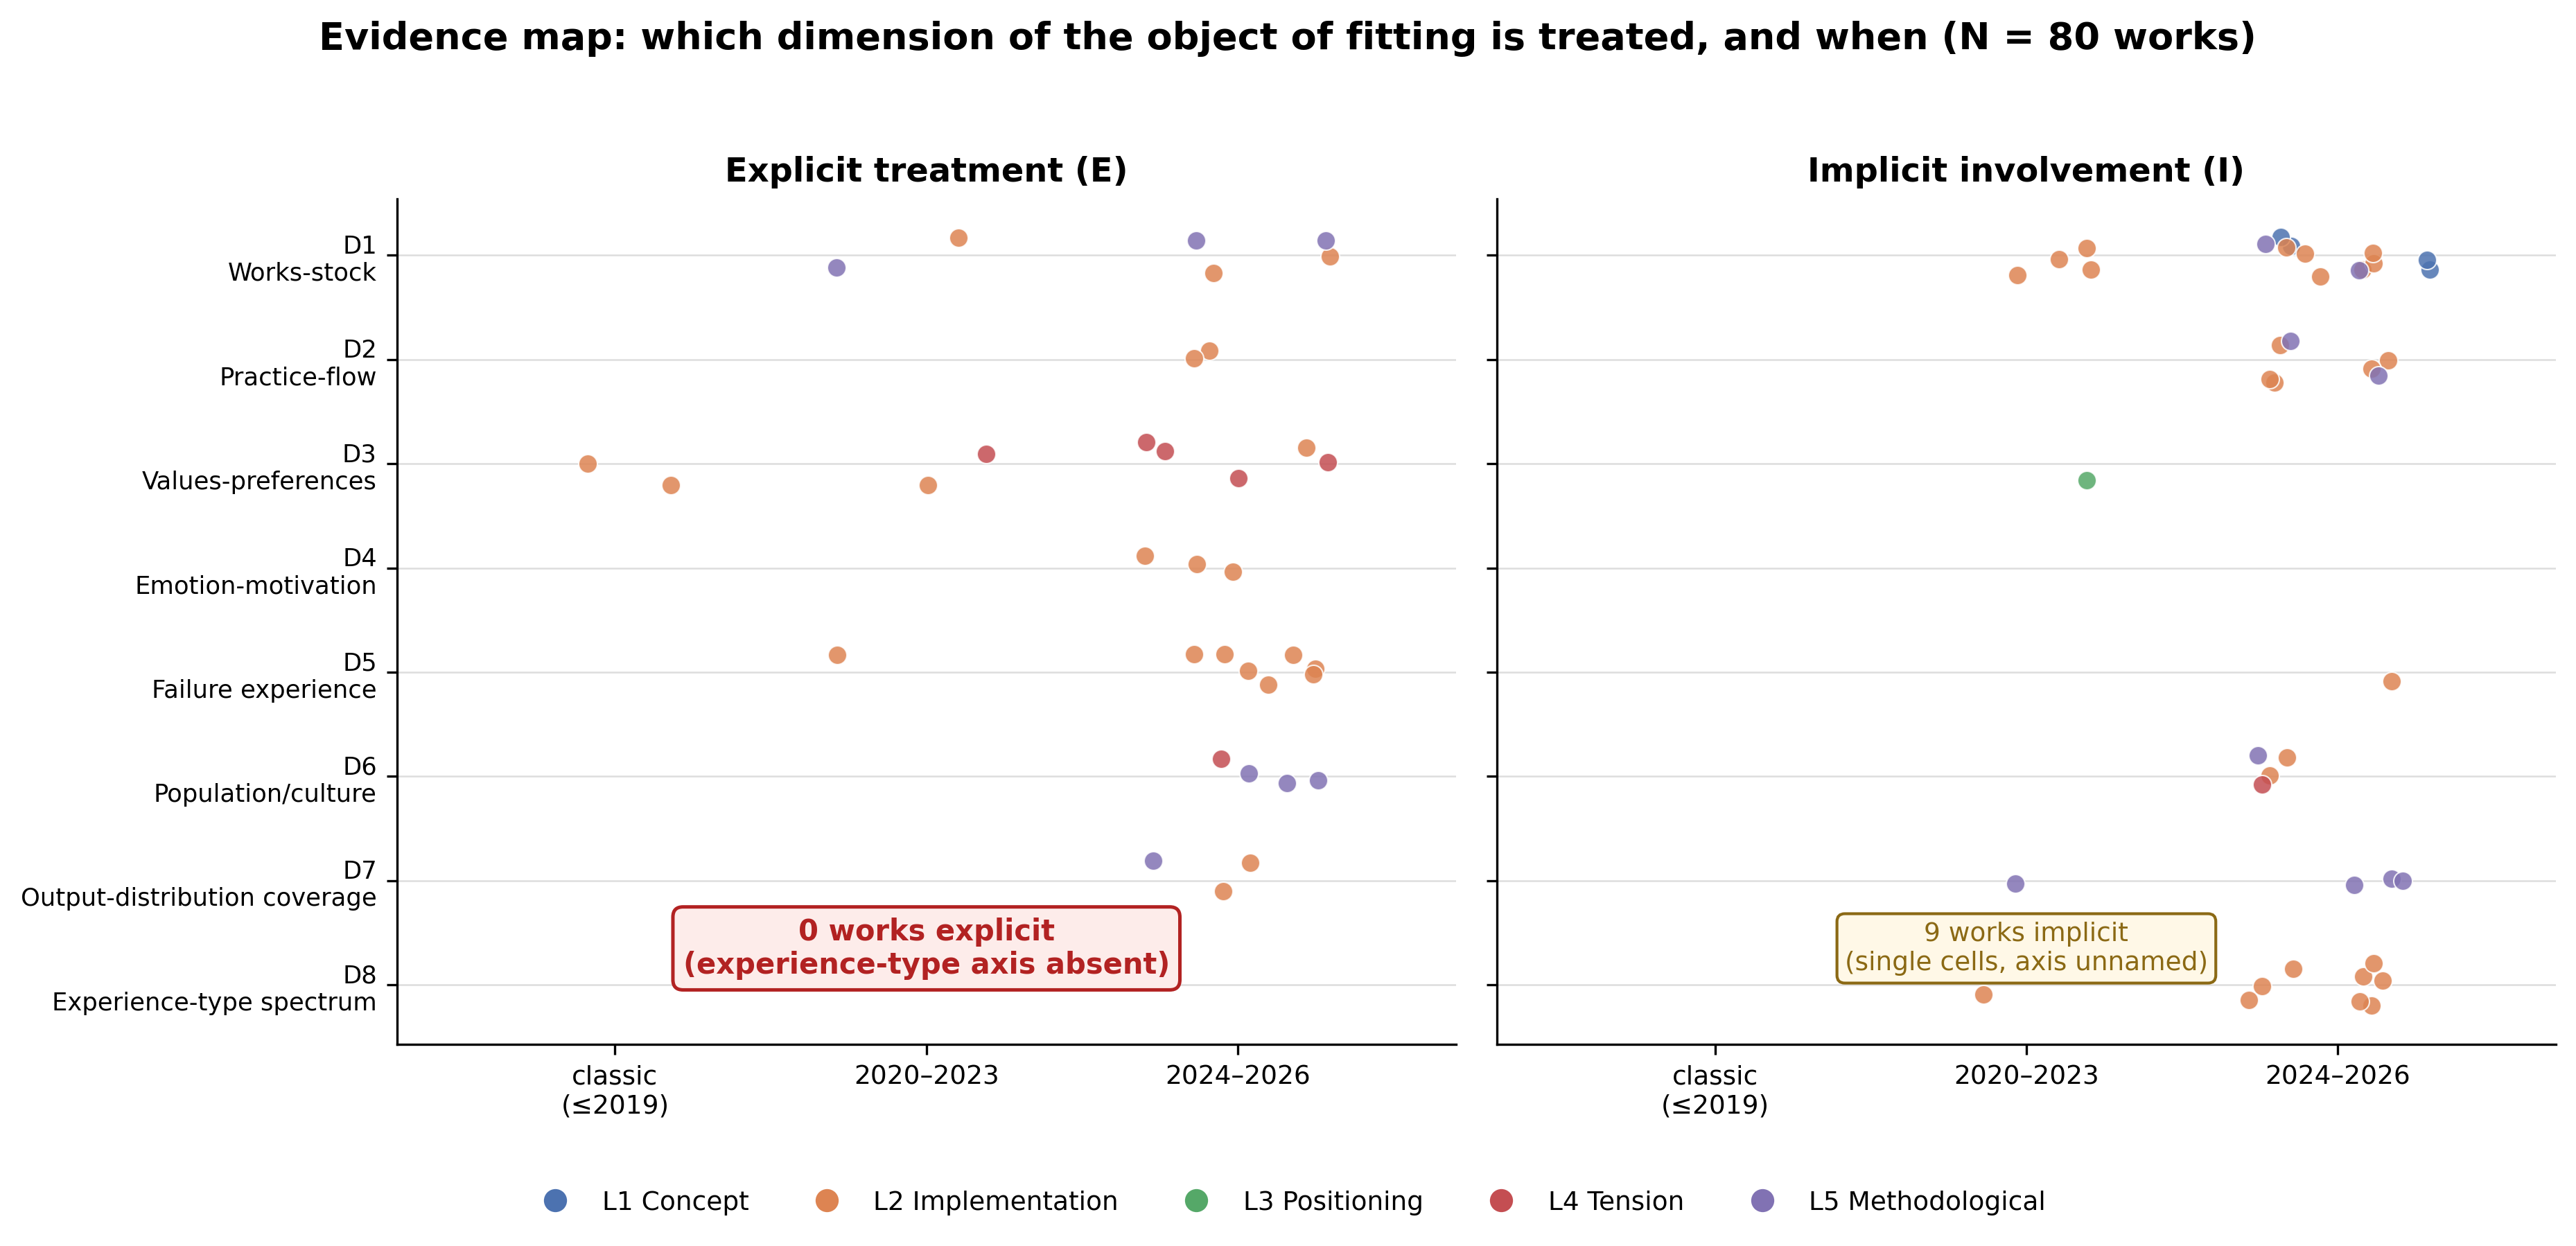
\includegraphics[width=\textwidth]{fig2_evidence_map.png}
\caption{Evidence map of the 80-work corpus (year stratum $\times$ dimension; point color = layer L1--L5). Left panel: explicit treatment (E). Right panel: implicit involvement (I). The D8 row is empty in the left panel --- zero works, with the red-box annotation ``0 works explicit (95\% CI $[0, 4.5\%]$)'' --- while the same row carries nine implicit points in the right panel (``single cells touched, axis never named'').}
\label{fig:evidencemap}
\end{figure}

\begin{table}[t]
\centering
\caption{Stance distribution (A1 $\times$ A2, counts of works).}
\label{tab:stance}
\begin{tabular}{lrrrrr}
\toprule
A1 $\backslash$ A2 & augment & substitute & anti\_tool & na & Total \\
\midrule
support       & 1 & 0 & 1 & 16 & \textbf{18} \\
deny          & 0 & 0 & 0 & 3  & \textbf{3} \\
na            & 9 & 1 & 2 & 47 & \textbf{59} \\
\midrule
\textbf{Total} & \textbf{10} & \textbf{1} & \textbf{3} & \textbf{66} & \textbf{80} \\
\bottomrule
\end{tabular}
\end{table}

Marginals: A1 support 18 / deny 3 / na 59; A2 augment 10 / substitute 1 / anti\_tool 3 / na 66. The map's a-priori hypotheses were supported with one instructive refinement: all five training/system technical reports are A1-\emph{na} (DeepSeek-V4.1 \cite{deepseek2026v41}, MiMo-V2.6 \cite{xiaomi2026mimo}, GLM-5 \cite{zai2026glm5}, Llama 3 \cite{grattafiori2024llama3}, DeepSeek-R1 \cite{deepseek2025r1}) --- technical reports do not discuss fitting, though official \emph{empirical} reports can (the interpretability finding \cite{anthropic2026emotions} is A1-support); cognitive-empirical works concentrate on support (4/5); the superhuman-achievement line denies (2/2, plus one conceptual denial \cite{imeri2025benefits}); and the collapse/coverage line splits: all three works treat output distribution explicitly (D7=E: the hivemind study \cite{jiang2025hivemind}, model collapse \cite{shumailov2024collapse}, Spectrum Tuning \cite{sorensen2025spectrum}), with A1 support for the empirical collapse evidence \cite{jiang2025hivemind} and \emph{na} for the dynamics and methodology works \cite{shumailov2024collapse, sorensen2025spectrum} --- the coverage line does not assert ``fitting humans,'' it measures distributional consequences.

The decoupling design resolved the anticipated mixed cases: the Turing Trap is A1-support $\times$ A2-augment (route-level scope recorded); Vallor is A1-support $\times$ A2-anti\_tool (critical of the \emph{quality} of the fit, not its occurrence); the hivemind study is A1-support $\times$ A2-\emph{na}. Suleyman's works split by document (CR2 rule): the 2023 book is substitute-positioned \cite{suleyman2023coming}; the September 2026 statement set is augment-positioned \cite{suleyman2026personable}.

\begin{figure}[t]
\centering
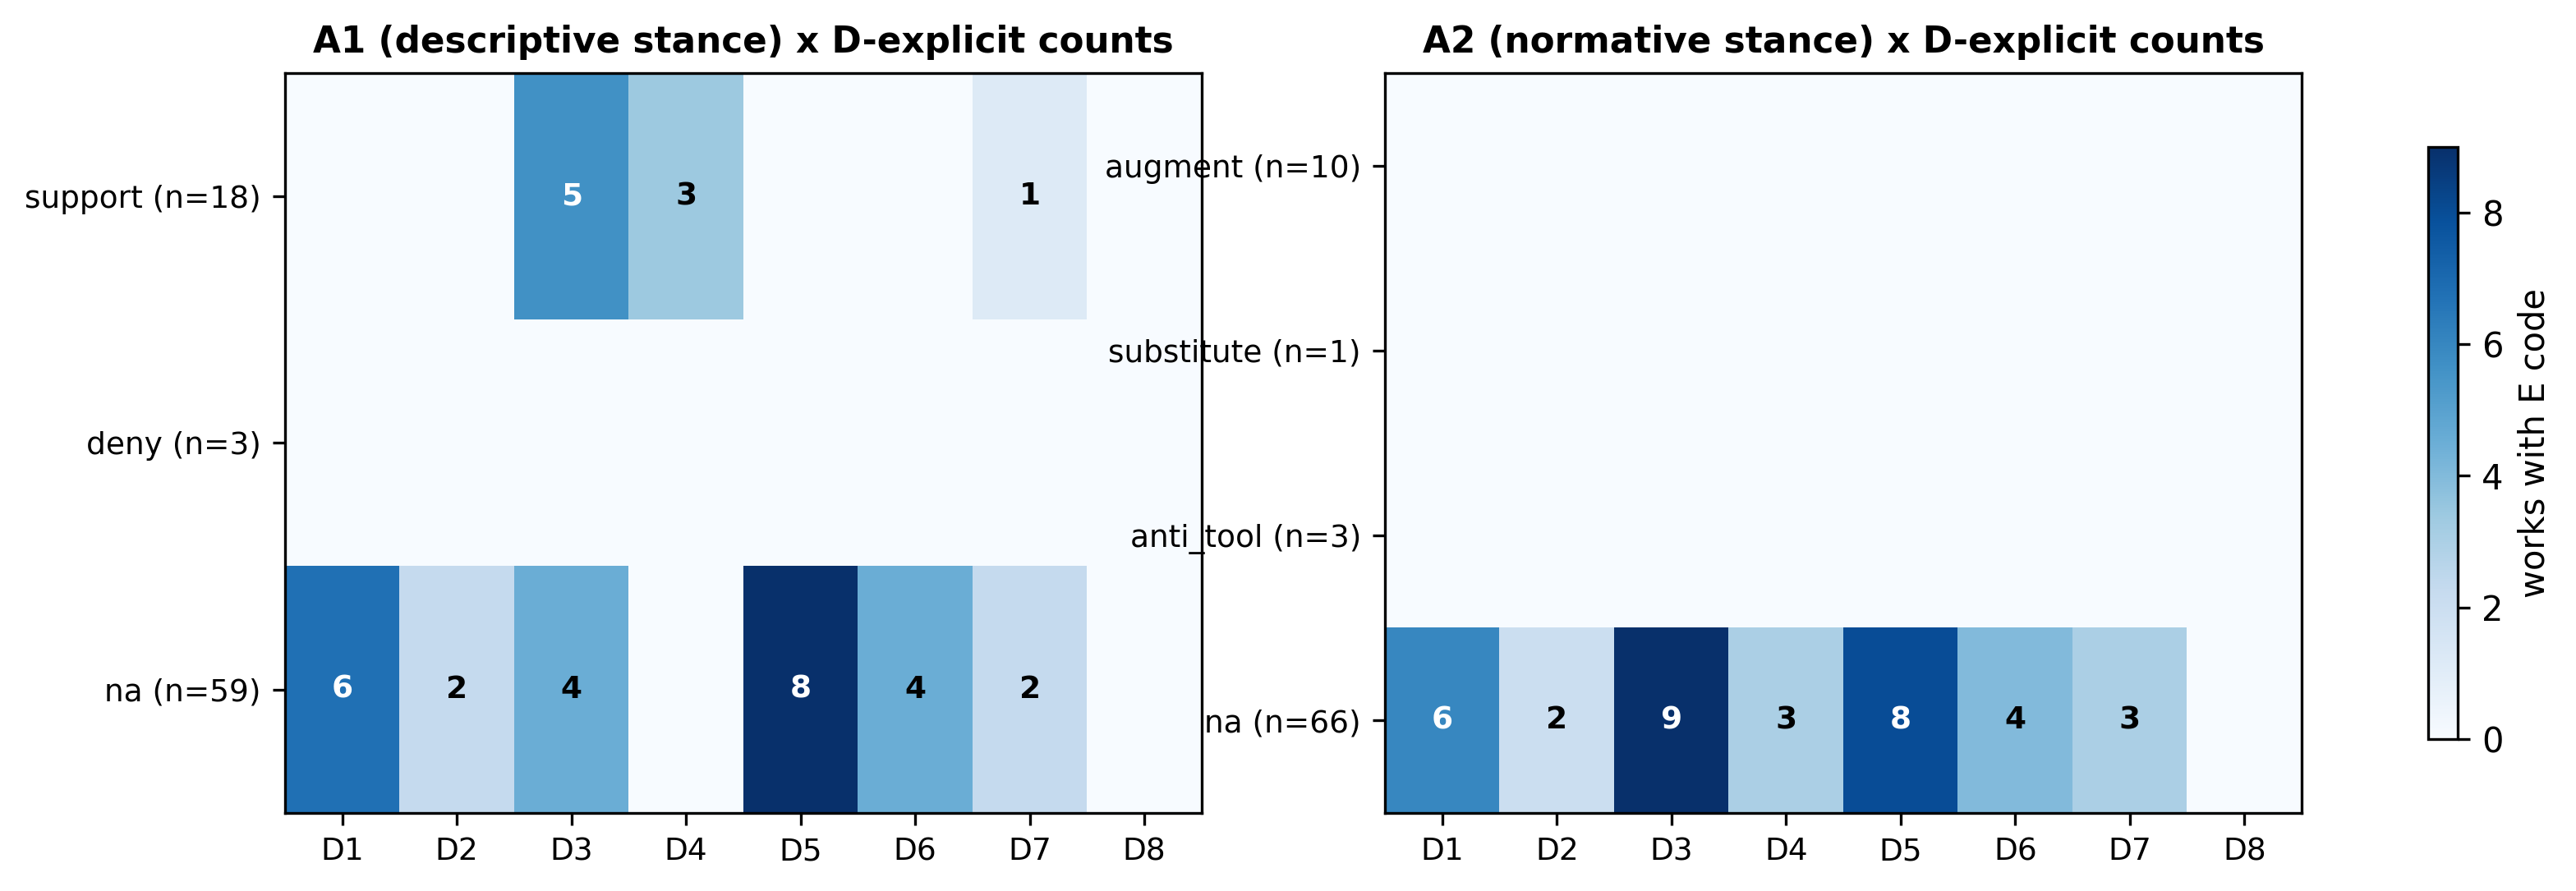
\includegraphics[width=\textwidth]{fig3_stance_dimension_heatmap.png}
\caption{Stance $\times$ dimension heatmaps (counts of explicit-E works). Left: descriptive stance A1 $\times$ dimension. Right: normative stance A2 $\times$ dimension. The all-zero \emph{deny} row (left) and the all-zero \emph{substitute} row (right) visualize the structural finding below: framework-level denial and subject-substitution advocacy engage in no dimension-level engineering.}
\label{fig:heatmap}
\end{figure}

The structural finding deserves its own sentence: the \emph{deny} row (left panel of Figure~\ref{fig:heatmap}) is entirely empty, as is the \emph{substitute} row (right panel). Descriptively and within this corpus: none of the three A1-deny works participates in any dimension-level engineering (0/3 with any dimension code, explicit or implicit), against 16/18 among A1-support works --- denial operates at the framework level, not the design level. (Exploratory cross-tabulations for these contrasts are reported in the supplementary analysis materials released with the repository using Fisher's exact tests, uncorrected and non-generalizing; we deliberately do not restate them here as inferential evidence, since a purposeful sample supports no population inference.)

\subsection{The principal result: an unnamed axis}\label{sec:unnamed}

\begin{table}[t]
\centering
\caption{Fitting-object dimensions: frequency of explicit (E), implicit (I), and absent ($\dminus$) treatment.}
\label{tab:dimensions}
\begin{tabular}{lrrrrr}
\toprule
Dimension & E & I & $\dminus$ & \%E & \%E or I \\
\midrule
D1 works-stock                        & 6 & 16 & 58 & 7.5\%  & 27.5\% \\
\textbf{D2 practice-flow}             & \textbf{2} & 7 & 71 & \textbf{2.5\%} & 11.2\% \\
D3 values-preferences                 & 9 & 1  & 70 & 11.2\% & 12.5\% \\
D4 functional emotion-motivation      & 3 & 0  & 77 & 3.8\%  & 3.8\% \\
D5 failure experience                 & 8 & 1  & 71 & 10.0\% & 11.2\% \\
D6 population/culture (who)           & 4 & 4  & 72 & 5.0\%  & 10.0\% \\
D7 output-distribution coverage       & 3 & 4  & 73 & 3.8\%  & 8.8\% \\
\textbf{D8 experience-type spectrum}  & \textbf{0} & \textbf{9} & 71 & \textbf{0.0\%} & \textbf{11.2\%} \\
\bottomrule
\end{tabular}
\end{table}

\textbf{D8-explicit $=$ 0/80 (0.0\%)}, exact binomial (Clopper--Pearson) 95\% CI $[0.0\%, 4.5\%]$, rule-of-three upper bound $\approx 3.8\%$. The result is insensitive to confidence: excluding all 8 low-confidence works leaves D8-E $=$ 0/72, CI $[0.0\%, 5.0\%]$. The contrast modality matters as much as the zero: \textbf{D8-implicit $=$ 9/80} --- the failure-data works (LEMA \cite{an2023lema}, PRM800K \cite{lightman2024verify}, SPAR \cite{spar2026f26}, ETO \cite{song2024trial}, UltraInteract \cite{yuan2024advancing}, DeepSeek-V4.1 \cite{deepseek2026v41}, MiMo \cite{xiaomi2026mimo}, GLM-5 \cite{zai2026glm5}) and the hivemind study \cite{jiang2025hivemind} each touch a \emph{single cell} of the type space (failures only, or the average only); none names or operationalizes experience type as a coverage axis. The finding is thus precisely stated: \textbf{the topic is touched; the axis is never named.} This is the quantified form of the theory's third-coverage-axis claim.

\paragraph{Absence-search procedure.}
A zero count is only as strong as the search behind it. We ran a pre-specified, logged absence-search (8 query families across arXiv full-history, ACL Anthology domain search, and Chinese-language web search; log in Appendix~\ref{sec:appendix-absence}): all hits were screened against the D8-E criterion (the experience-type dimension \emph{named} as a coverage/sampling axis \emph{and} used to design data, experiments, or metrics). No hit satisfied the criterion; eight families of near-misses were logged with reasons. The nearest misses are instructive: agent-experience benchmarks treat ``experience'' as the agent's own prior episodes (temporal, not typed); data-mixture lines optimize domain weights; and --- the closest pair --- two 2026 works shape the \emph{diversity of model errors in machine rollouts} as an exploration/RL signal \cite{baek2026dfuser, liu2026leveraging}. That last pair shows the third axis being approached from the machine side while the human-data side remains at zero; our claim is accordingly restricted to ``as a coverage axis over human-practice data,'' and would be falsified by works that operationalize it. A re-check of the search on 2026-10-19, after the coding freeze, sharpens rather than dissolves the zero. Typed coverage of \emph{culture and population} has now been operationalized at industrial scale --- a tagging framework and 5.6-million-sample tagged corpus measuring cultural-signal coverage across pretraining, fine-tuning, alignment, and reasoning stages \cite{sahu2026culturefunnel} --- which on this paper's coordinates is the population axis (D6), not the experience-type axis (D8). Typed \emph{trajectory} diversity is operationalized in RL post-training with user-specified type distributions \cite{fu2026tjpo} --- over the model's own rollouts, the machine side again. And ``diversity of the training data'' now appears as a named factor in entropy-collapse analyses of RLVR \cite{jin2025entropy} --- as prompt-set diversity within an RL run, not as coverage design of the human-practice corpus. The pattern across all three: the axes adjacent to experience type are acquiring operationalizations, and the experience-type axis over human practice remains the one neither named nor measured. Figure~\ref{fig:evidencemap} displays the combined result: the empty D8 row in the explicit panel against its nine implicit points --- the axis touched, never named.

\subsection{The temporal pattern}\label{sec:temporal}

\begin{table}[t]
\centering
\caption{Explicit treatment by year stratum (with D8-implicit for contrast).}
\label{tab:temporal}
\begin{tabular}{lrrrr}
\toprule
Dimension $\times$ modality & $\leq$2019 & 2020--2023 & 2024--2026 & Total \\
\midrule
D1 explicit       & 0 & 2 & 4 & 6 \\
D2 explicit       & 0 & 0 & \textbf{2} & 2 \\
D7 explicit       & 0 & 0 & 3 & 3 \\
\textbf{D8 explicit} & \textbf{0} & \textbf{0} & \textbf{0} & \textbf{0} \\
D8 implicit       & 0 & 1 & 8 & 9 \\
\bottomrule
\end{tabular}
\end{table}

The three-row contrast narrates the theory. Works-as-stock is the \emph{mature} program: D1-E works appear continuously 2022--2026 (the data-wall analysis \cite{villalobos2022data}, mixture optimization \cite{xie2023doremi, ye2024data}, flagship corpus design \cite{grattafiori2024llama3, penedo2024fineweb}). Output-distribution coverage is the \emph{arriving} awareness: D7-E first appears in 2024 \cite{shumailov2024collapse} and consolidates \cite{jiang2025hivemind, sorensen2025spectrum}. The experience-type axis is the \emph{missing} third: 0 in every stratum. Practice-as-flow is \emph{nascent, not established}: D2-E $=$ 2/80, both from 2026 --- the employee failure-submission stream at DeepSeek (``we collect negative feedback and model failure cases submitted by internal employees at scale'' \cite{deepseek2026v41}) and the concurrent stock/flow engineering essay \cite{gharbi2026model}. We stress the wording: two works constitute a beginning, not a trend.

Two qualifications from the map. First, the WEIRD-paradox unit \cite{zhou2025should}: increasing cultural representativeness of training data can \emph{amplify} reproduction of discriminatory views --- representing \emph{who} does not fix \emph{what}. The coverage problem is thus two-axes-known-and-unsolved, not two-axes-solved, which is exactly the space the third axis enters. Second, an exploratory structural observation (descriptive, within-corpus only): explicit-dimension engineering concentrates in A1-\emph{na} works (23 with at least one explicit dimension, against 9 among A1-support works). Combined with the empty deny row of Section~\ref{sec:stance}, the pattern is a decoupling: those who debate whether AI fits humans mostly do not engineer coverage, and those who engineer coverage mostly do not debate it. This decoupling is the quantitative footprint of the gap stated in Section~\ref{sec:intro} --- the missing connective proposition.

\subsection{Limitations of the evidence map}\label{sec:maplimits}

A skeptical reviewer should accept these limits. (i) \textbf{No population inference}: the corpus is purposefully sampled with quota strata; all claims are ``within this corpus.'' (ii) \textbf{Single coder}: the pre-registered blind re-coding returned overall $\kappa$ = 0.731 (Section~\ref{sec:method}), with two standing caveats --- the second coder is an AI agent of the same model family as the original coding assistant, a weaker form of independence than a human second coder, and one sampled work was codeable only at title level; the mitigations remain the published codebook, mandatory quote anchors, and the public boundary-case log, which now includes all 23 re-coding disagreements. (iii) \textbf{Strict saturation not reached}: the corpus was filled to the 80-work cap with the shortfall reported. (iv) \textbf{Absence claims are procedure-bounded}: 0/80 plus an 8-query absence-search is strong within its window (closed 2026-10-15), not eternal. (v) \textbf{Core claims are confidence-independent} (Section~\ref{sec:unnamed} sensitivity), but 8 units remain low-confidence pending the final corpus freeze. (vi) The map disciplines the \emph{descriptive} claims; the \emph{normative} stance of Section~\ref{sec:position} is an argued choice, not a map result. Concurrent works are flagged, coded in a dedicated single-row supplement (Table~\ref{tab:gharbi}), and excluded from the gap claims; the full demarcation is consolidated in Section~\ref{sec:concurrent}.

\section{Adjacent Frameworks and Consolidated Demarcation}\label{sec:concurrent}

This section fixes the theory's position against its neighbors on three fronts: concurrent works that share the stock/flow diagnosis, adjacent frameworks that neighbor the theory's claims, and architecture-side programs that share the diagnosis while prescribing different layers of the machine.

Two concurrent works are flagged and demarcated. \textbf{Gharbi's SSRN essay} \cite{gharbi2026model} analyzes nine escape routes from the data wall using an explicit stock/flow engineering framing and identifies a ``verifier wall'' behind the data wall --- the closest published phrasing to our temporal clause. The demarcation is sharp: it is data engineering. It contains no works-versus-practice ontological distinction, no full-spectrum $\times$ full-course coordinate system, no coverage axes, and no tool positioning; its flow is a supply chain, not a fitting object. Its D1-E/D2-E codes are reported in a dedicated single-row supplement (Table~\ref{tab:gharbi}), and it is not counted against the theory's gap claims. \textbf{Fenoglio's asymmetric-communication essay} \cite{fenoglio2026asymmetric} argues that LLM outputs acquire meaning within human practice under an asymmetry of commitment --- a meaning-side theory with no fitting program, no augmentation positioning, and no coordinate system. A third concurrent work reaches the same stock/flow conclusion from economics: a theory of the human-data market models structured human-data work --- evaluation, rubric judgment, auditing, exception handling --- as a persistent labor \emph{flow} that builds a depreciating capability stock \cite{ansari2026nolastmile}; it concerns the market for the flow, not the fitting of it, and supplies no coverage axes and no training-data design. Cross-disciplinary convergence without overlap. None of the three anticipates the temporal clause's three-element combination (practice-not-works, full-spectrum $\times$ full-course, stock-wall/flow-no-wall), which no prior work states as of the window close.

A second family of neighbors is architectural rather than humanistic or economic: programs that share the diagnosis --- static corpus fitting will not carry machine intelligence to generality --- while prescribing a different layer of the machine. LeCun's world-model program (JEPA: prediction in representation space, driven by intrinsic objectives rather than text corpora) \cite{lecun2022path} rebuilds the \emph{prediction} layer; Zhu Songchun's value-driven program --- ``erect a heart for machines,'' instantiated by the toddler-level agent Tongtong with built-in value drives, evaluated in a Utility--Value dual space \cite{zhao2024heart} --- rebuilds the \emph{architecture} layer, fitting value structure as innate content. The present theory prescribes neither layer: it is a claim about the \emph{data} layer --- what the training signal should be. The three programs occupy orthogonal axes (architecture $\times$ prediction objective $\times$ fitting object) and are combinable in principle; what neither architecture-side alternative can see is the fitting-object axis itself, and that is where the audit's 0/80 sits. The layering also fixes a naming disambiguation: this is not a human-centered-design proposal (governing \emph{for whom} systems are built) and not a mind-fitting proposal (fitting human cognitive structure or values as content into the machine); it changes what is fitted, not who is served or what architecture runs --- a distinction the theory's name does not announce, and therefore stated here once, explicitly.

\begin{table}[t]
\centering
\caption{This theory versus adjacent frameworks.}
\label{tab:frameworks}
\small
\begin{tabular}{p{0.30\textwidth}p{0.31\textwidth}p{0.31\textwidth}}
\toprule
Framework & Provides & Lacks (what this theory adds) \\
\midrule
Cultural technologies \cite{farrell2025cultural, yiu2024transmission} & Descriptive classification: LLMs inherit human symbolic structure & Temporal distinction (works vs.\ practice); coverage axes; data-methodological consequences \\
\addlinespace
Critical phenomenology (mirror) \cite{vallor2024mirror} & Warning: distorted reflection reshapes human self-understanding & Constructive account of faithful fitting; spectrum/course coordinates; boundary conditions \\
\addlinespace
Augmentation economics \cite{brynjolfsson2022turing, engelbart1962augmenting, shneiderman2022human} & Normative goal: complements over substitutes; design point (control $\times$ automation) & Fitting ontology (why imitation-as-\emph{means} differs from imitation-as-\emph{goal}); termination boundaries \\
\addlinespace
Stock/flow data engineering \cite{gharbi2026model} (concurrent) & Supply-side analysis: escape routes, verifier wall & Practice ontology; third coverage axis; tool positioning \\
\addlinespace
World-model architectures \cite{lecun2022path} & Prediction-side answer: JEPA world model, intrinsic objectives & Fitting-object claim; coverage axes; tool positioning \\
\addlinespace
Value-driven developmental AGI \cite{zhao2024heart} & Architecture-side answer: innate value drives (Tongtong; Utility--Value dual space) & Fitting-object claim (data layer); orthogonal and combinable \\
\bottomrule
\end{tabular}
\end{table}

\section{Tensions and Boundaries}\label{sec:tensions}

The theory's fourth layer addresses where the fit strains against itself and where it stops.

\paragraph{Value pluralism: whose spectrum?}
The full spectrum is a \emph{who} question before it is a \emph{what} question. The alignment literature has long recognized that value fitting underdetermines whose values \cite{gabriel2020values}; the pluralistic-alignment roadmap operationalizes pluralism across populations \cite{sorensen2024roadmap}; social-choice critiques show that preference aggregation embeds contested normative commitments (utilitarian vs.\ leximin aggregation over heterogeneous feedback) \cite{park2024rlhf}; aggregation-problem analyses catalog the failure modes \cite{baum2025aggregation}; and collective-constitutional experiments with ${\sim}1{,}000$ (US) participants demonstrate both the feasibility and the \emph{geographic narrowness} of current collective processes \cite{huang2024collective}. The spectrum axis does not dissolve this tension --- it inherits it. A full-spectrum fit still requires an aggregation decision, which is why Section~\ref{sec:implications} treats governance as a question in its own right.

\paragraph{The subjectivity boundary: never personhood, never phenomenal fitting.}
The sharpest live clash in the corpus is instructive. Anthropic's model-welfare program asks whether models may deserve moral consideration \cite{anthropic2025welfare}; Suleyman's September 2026 statements publicly reject that route: AI should be personable --- with personality --- but never granted personhood \cite{suleyman2026personable}. We read this as an unexpected alliance across opposing camps, and we hold the boundary on independent grounds: never grant personhood and never fit phenomenal states are two faces of one boundary coin. The fitting target includes functional emotion-motivation structure --- and interpretability evidence for causally functional emotion concepts \cite{anthropic2026emotions} confirms that this layer \emph{is} being fitted --- but the theory's boundary sits exactly at the functional layer: no claims about felt experience are made, licensed, or needed. The mirror critique \cite{vallor2024mirror} supplies the complementary warning: the danger of a fitted mirror is not that it feels, but that its reflection restructures what humans take themselves to be.

\paragraph{The boundary argument closed: cheap, dangerous, unnecessary.}
Three independently available premises close the argument for this boundary. (i) \emph{Personhood is cheap}: standing is not capability-graded --- persons with severe cognitive impairment hold it in full; a narrative self requires memory continuity, value consistency, and relational correction, not horsepower. If personhood is internal structure interactively completed by social practice, then a functional personality structure is, in principle, architecturally constructible, and withholding the grant is not a capability judgment --- ``grant it once it is smart enough'' is structurally confused. (ii) \emph{The dangerous conjunction is status $\times$ capability, not capability alone}: AlphaFold surpassed every human teacher at protein folding --- a local B2 event --- without creating a control problem, because a heartless tool's outputs remain checkable by institutions of verification. Capability beyond every teacher removes the arbiter (B2: the reference exhausts); personhood supplies its own direction (own meaning, own values --- an objective of its own). Neither alone is fatal; the conjunction is the sufficient condition for uncontrollability. Read through this theory, the control problem is a question about status, not about horsepower. (iii) \emph{The boundary costs nothing}: everything humans need from the system --- intentions read, corrections absorbed, misunderstandings repaired --- is delivered at the functional layer; the phenomenal and standing layers add nothing to human ends. Cheap to draw, load-bearing where it matters, costless to hold: the boundary's three sentences --- fit functional personality structure, never fit phenomenal states, never grant standing --- follow from these premises at once.

\paragraph{The tacit-dimension objection: immune at the goal level, open at the functional level.}
The strongest philosophical objection leaves data design aside: if the core of intelligence is embodied and tacit --- skill where ``we know more than we can tell'' \cite{polanyi1966tacit}, understanding rooted in a lived body \cite{dreyfus1992what} --- then no fitting reaches it, and practice-fitting at most approaches a functional shell. The theory splits this objection in two. At the goal level it is inert by construction: the tool stance promises no phenomenal or replicative equivalence; the fitting target is functional service capability, and the subjectivity boundary above already draws that line. At the functional level the objection becomes an open empirical question the theory can index rather than dodge: whether functional cognitive empathy --- reading unstated intentions, absorbing corrections, repairing misunderstandings --- is learnable from the practice flow is precisely what the population and expertise axes of the coverage space can measure, cell by cell, on evaluator-graded tasks. The objection thus lands not as a refutation but as a research program for which the theory already has coordinates.

\paragraph{Four termination boundaries.}
The temporal clause ends where its terms end; the theory fixes four boundaries explicitly.
\begin{itemize}
\item \textbf{B1 --- End of the practicing subject.} The flow regenerates with life; the fit has no object beyond the last practice. (An existential boundary, not an engineering one.)
\item \textbf{B2 --- Fitter overreach.} If the fitter surpasses every teacher --- call it ASI --- the fitting relation exhausts itself: there is no human practice left to fit that is not already behind it. The theory is about AGI as a human-referential concept and is deliberately silent beyond this boundary, except to mark it. The two demands fixed in Section~\ref{sec:concept} meet their bounds differently: generality is bounded externally (B1, B3, B4), while height terminates its own reference --- exactly at this boundary.
\item \textbf{B3 --- Institutional boundary.} Law, privacy, and consent bound what may be collected; and the normative stance of Section~\ref{sec:position} reciprocally defines the \emph{water rights} over the flow --- the tool stance constrains not only what AI is for but what may be taken. (The pluralism tension above lives inside this boundary.)
\item \textbf{B4 --- Self-referential contamination.} Once AGI is woven into daily life, the practice being collected is already dyed by AGI: the fitting target is changed by the act of fitting --- the mirror enters the room it reflects. This is model collapse's new form in a flow regime \cite{shumailov2024collapse}: not recursion on a static stock but contamination of a live stream. The mitigation is engineering, not prohibition: stratified provenance tagging of native versus AI-mediated practice (a protocol component sketched for future work).
\end{itemize}

\paragraph{Falsifiability.}
The theory names its own falsifiers. If the flow side is shown to have a hard wall isomorphic to the stock wall (e.g., a principled lower bound defeating continual learning), or if full-spectrum fitting provably collapses to the mean at any scale, the temporal clause is weakened to a heuristic. If explicit experience-type coverage appears frequently in neutral literature, the third-axis gap claim (0/80) fails --- the adjacent operationalizations arriving in 2026 (population-axis cultural coverage \cite{sahu2026culturefunnel}; trajectory-type diversity \cite{fu2026tjpo}; RL prompt-set diversity \cite{jin2025entropy}) do not yet constitute that failure, and the distinction is drawn where the result is stated (Section~\ref{sec:unnamed}). The D2-E count (2/80) fails as evidence if practice-flow data streams prove unbuildable at production quality. These are stated so that the theory can lose.

\section{Methodological Implications}\label{sec:implications}

From theory to method: for each of the three questions below, we state the problem, the current state visible in the map, and the shape of the answer. Full protocols are left to future work.

\paragraph{Distribution $=$ full-spectrum coverage.}
In current practice, diversity exists in three identities: as a regression variable (domain-weight optimization \cite{xie2023doremi, ye2024data}, with implicit multilingual quotas such as Llama 3's 8\% \cite{grattafiori2024llama3}); as local heuristics (persona-conditioned synthesis at billion scale \cite{ge2024scaling}); and as the casualty of quality filtering (educational-corpus curation discards on the order of 92\% of the raw web \cite{penedo2024fineweb}). The turn toward coverage as an explicit post-training objective --- distributional coverage restored against instruction-tuning collapse \cite{sorensen2025spectrum} --- is the right kind of move, but it covers the \emph{output distribution} axis; the population axis has its own line (multilingual curation, e.g., 65-language instruction collections \cite{singh2024aya}; cultural-signal coverage now tagged at industrial scale \cite{sahu2026culturefunnel}); and the experience-type axis is at 0/80 (Section~\ref{sec:unnamed}). The WEIRD paradox \cite{zhou2025should} warns that naive population quotas backfire (representing \emph{who} $\neq$ fixing \emph{what}), so full-spectrum coverage must integrate the axes rather than stack quotas. We use ``coverage,'' not ``quota,'' deliberately. A concrete pathology marks the stakes: sycophancy is what fitting a single cell of the coverage space looks like. A pipeline that ingests only instant user-satisfaction signals --- population reduced to the user, outcome to success, no evaluator tier, no professional calibration --- is not merely ``at risk of'' sycophancy; the theory reads the disease as coverage deficiency made visible, and its antidote is the missing cells: evaluator-population signals and professional-tier judgment \cite{yu2026methodology}.

\paragraph{Production $=$ perpetual collection protocol.}
The flow side requires an organizational apparatus, and its precedents are visible: employee-submitted failure cases at scale \cite{deepseek2026v41}; failure-reflection and error-retention practices in agentic training \cite{xiaomi2026mimo, zai2026glm5}; and, at the widest institutional scale so far, consumer terms that route ongoing chat and coding sessions into training under opt-out \cite{anthropic2025consumerterms} --- a tap into practice-flow rather than works-stock. The protocol components, defined here and left to future work: a collection protocol with failure cases as first-class data; toxicity cleaning that distinguishes true failures from reward-hacking pseudo-failures (the audit's boundary condition \cite{yu2026failure}); a three-part record structure (error type, root cause, correction); and collapse guards for any synthetic augmentation, now with quantified anchors --- a single real datapoint per retraining step provably prevents closed-loop collapse in exponential families \cite{jangjoo2026lost}, convergence under contamination is governed by the real-data fraction \cite{wang2026guarantees}, accumulation preserves what replacement destroys (independently reconfirmed as a ``screening'' collapse that precedes model collapse \cite{zhang2026screening}), and degradation arrives asymmetrically --- already-strong skills reinforced while weak ones decay \cite{luo2026polarization} --- so admixture floors must be typed by capability, not set globally. The binding constraint is not collection but \emph{absorption}: practice regenerates daily while model snapshots update on cycle --- the \emph{fitting lag} --- and the stability--plasticity dilemma for agents remains unresolved \cite{wu2026agentdice}. Absorption is nonetheless becoming practical: time-incremental continued pretraining without catastrophic forgetting is demonstrated at open-weight scale \cite{oncel2026timeincremental}, and self-generated replay nearly eliminates forgetting in parametric memory \cite{marek2026replay} --- which makes the absence of disclosed per-tier lag metrics the binding transparency gap rather than a research unknown. The map codes the absorption-side works as D2-implicit: their data source is not (yet) specified as practice-flow. (After the evidence window closed, reporting indicated that frontier labs now run tens of thousands of RL training exercises in parallel, with models configuring, monitoring, and grading them \cite{nolan2026fortune} --- the scaling story's center of gravity moving from data-stock to RL-process, which is exactly where the flow question lands.)

\paragraph{Governance $=$ pluralistic aggregation and institutions.}
Who aggregates the spectrum, who licenses the flow, and who adjudicates failure: the aggregation toolbox spans social-choice mechanisms \cite{park2024rlhf}, multi-constitution processes \cite{huang2024collective}, persona-conditioned generation \cite{ge2024scaling}, and sovereign local models; licensing confronts the concentration of provenance rights in a few large publishers; and the verifier question --- who certifies that a failure is a failure --- is the load-bearing element of the entire training loop \cite{yu2026failure, gharbi2026model}. B4's mitigation (native vs.\ AI-mediated provenance stratification) is likewise an institutional demand on the data infrastructure, not merely a labeling convention --- and it is becoming an engineering feasibility: statistical-watermark detection, boosted by signature filtering, now reaches 78--99\% accuracy at the low-entropy signal strengths where it previously failed \cite{hong2026signature}.

\section{Conclusion}\label{sec:conclusion}

This paper has argued the three-layer thesis of the human-referential fitting theory: AGI is a philosophical concept whose reference frame is human practice; its implementation is the fitting of that practice --- works-as-stock being the mature form of the static misreading, practice-as-flow the beginning of the correct one; and its proper position is the augmentative tool, a normative choice that institutions must continuously defend. The evidence map makes the theory's claims quantifiable: a corpus of 80 works in which the experience-type coverage axis is never named (0/80; 95\% CI $[0.0\%, 4.5\%]$), practice-as-flow is explicit in only two works (both 2026), and stance and object decouple across the literature --- the descriptive, the normative, and the methodological literatures mature separately, unconnected by the one proposition that needs all three. The theory's contribution is that proposition, its coordinate system, its boundaries, and its named falsifiers.

We end where the theory begins, with the sentence that separates the two futures of the field --- accumulating archives until the wall, or fitting practice as it regenerates:

\begin{quote}
\textbf{The object of fitting is not humanity's works but its practice --- the full spectrum and the full course of human experience. The stock has a wall; the flow does not.}
\end{quote}

Whether the flow is fitted well --- across the full spectrum, along the full course, under the four boundaries, toward augmentation --- is not a prediction to await but a program to execute. Its execution is left to future work.

\medskip
\paragraph{Data and code availability.}
The corpus (corpus\_v1, 80 works $\times$ 24 fields), the codebook, the absence-search log, all table CSVs, figures (300 dpi), and the single-file reproduction script (\texttt{analysis/coding\_data.py}; seed 20261015) are released with the paper's repository.
% TODO(user): insert repository URL and DOI (Zenodo) at release; The companion audit's full materials: DOI 10.5281/zenodo.23355929.
The companion audit's full materials: DOI 10.5281/zenodo.23355929.

\paragraph{AI-assistance disclosure.}
Following the practice of the companion audit paper: literature search, verification, coding, and drafting were conducted with AI assistance under the author's supervision and rule-governed protocol (codebook rules R1--R5, CR1--CR6; verification log in the supplementary analysis materials released with the repository); all coded claims carry verbatim or design anchors, and single-coder limitations are disclosed in Section~\ref{sec:maplimits}.

\paragraph{Conflict of interest.}
None declared. This research was conducted at an independent research institution (YYG Strategy Lab) with no external funding and no financial relationships with the organizations whose public documents are analyzed.

\appendix

\section{Absence-Search Log (Executed 2026-10-14)}\label{sec:appendix-absence}

The pre-specified, logged absence-search behind the D8-explicit $=$ 0/80 claim (Section~\ref{sec:unnamed}): eight query families across three engines (arXiv full-history; ACL Anthology domain search; Chinese-language web search). Screening criterion (both conjuncts required): (i) the experience-type dimension (success/failure $\times$ expert/novice $\times$ typical/marginal) named as a coverage/sampling/stratification axis; (ii) that axis used to design data, experiments, or metrics. Result: \textbf{0 passing works; eight near-miss families logged with reasons}. Representative hits are given with verifiable identifiers; the full log with all hits is released with the repository. A post-freeze re-check of the same search, executed 2026-10-19 and reported with the result it re-examines (Section~\ref{sec:unnamed}), again returned 0 passing works; the nearest neighbors it surfaced are demarcated there.

\begin{table}[h]
\centering
\caption{Absence-search log: eight query families, 0 D8-E hits.}
\label{tab:absence}
\footnotesize
\begin{tabular}{p{0.055\textwidth}p{0.29\textwidth}p{0.55\textwidth}}
\toprule
\# & Query family (engine) & Representative hits and registered near-miss reason \\
\midrule
Q1 & ``success and failure'' coverage training (arXiv) & Continual-pretraining merging (2511.02451); user-edit fine-tuning (NeurIPS 2025). Qualitative case analyses, no coverage-axis design. \\
Q2 & ``expert'' ``novice'' data mixture (arXiv) & SimInstruct (2508.04428) generates expert--novice dialogue as a \emph{data type}, not a mixture/coverage axis; mixture lines (2502.15950, 2607.01104, 2601.17858) optimize domain weights. \\
Q3 & ``experience type'' coverage (arXiv) & AhaBench (agents learning from prior episodes); VCR (AAAI 2025). ``Experience'' = the agent's own episodes (temporal), not a typed spectrum --- the nearest miss, logged item by item. \\
Q4 & ``error diversity'' curriculum (arXiv) & DiVERT (2406.19356, EMNLP 2024); GEC data-weighting. Error diversity for distractor generation/correction, not fitting-data coverage. \\
Q5 & ``typical'' ``edge'' spectrum coverage (arXiv) & Autonomous-driving edge-case surveys (2410.08491); corner-case generation. Typical-to-marginal operationalized for \emph{scenario testing}, not human-practice fitting data. \\
Q6 & Chinese web: success/failure case ratio; expert/novice coverage & LLM-training-data survey (2411.07715); press coverage of data bottlenecks. Only proposition-level hit is a T3 media source (motivation layer only, excluded under the first-party-source rule). \\
Q7 & success failure expert novice coverage data selection (ACL Anthology) & Data-selection line (Albalak 2402.16827; ACL 2025; LESS). Influence/quality as the axis; no experience-type axis. \\
Q8 & ``error diversity'' / ``failure diversity'' training coverage (arXiv) & \textbf{D-FUSEr} (ICML 2026, PMLR 306); \textbf{EDAS} (2605.17333). Both shape the error distribution of \emph{model rollouts} (machine-side diversity as exploration/RL signal), not human-experience-type coverage --- the most important near-miss pair: the third axis is being approached from the machine side while the human-data side remains at zero. \\
\bottomrule
\end{tabular}
\end{table}

\section{Supplement S1: Concurrent-Work Coding Row (Gharbi)}\label{sec:appendix-gharbi}

\begin{table}[h]
\centering
\caption{Supplement S1: dedicated single-row coding record for the concurrent stock/flow data-engineering essay (handled under the concurrent-work rule), reported separately and not counted against the theory's gap claims (Section~\ref{sec:concurrent}).}
\label{tab:gharbi}
\small
\begin{tabular}{p{0.16\textwidth}p{0.72\textwidth}}
\toprule
Work & W-038: Gharbi (2026), SSRN preprint 7479298 (2026-09-17) \\
\midrule
Codes & A1 = na; A2 = na; D1 = E; D2 = E; D2-explicit = True; concurrent = True; confidence = medium \\
Delimitation & Engineering stock/flow $\neq$ practice ontology: no works-vs-practice distinction, no full-spectrum $\times$ full-course frame, no coverage axes, no tool positioning \\
\bottomrule
\end{tabular}
\end{table}

\bibliographystyle{unsrtnat}
\bibliography{references}

\end{document}
